%% bare_conf.tex  (modified version)
%% 完整修正版，适用于 IEEE Transactions 格式
%%
%% 使用前请确保：
%%   - 替换占位作者信息
%%   - 准备 Figure_1.png 图片
%%   - 根据实际数据调整表格内容

\documentclass[journal]{IEEEtran}
\IEEEoverridecommandlockouts

% 引用包（自动压缩编号）
\usepackage{cite}
% 图片宏包
\usepackage{graphicx}
% 数学宏包
\usepackage{amsmath, amssymb}
% 表格增强
\usepackage{array}

% 自定义命令（可选）
\hyphenation{op-tical net-works semi-conduc-tor}

\begin{document}

% -------------------- 标题 --------------------
\title{Reinforcement Learning-Based Automatic Recommendation System for Limestone Slurry Feed Pump in Wet Flue Gas Desulfurization}

% -------------------- 作者 --------------------
\author{\IEEEauthorblockN{Kevin Zhang}
\IEEEauthorblockA{School of Communication and Information Engineering\\
Electronic Science and Technology\\
Xi'an University of Science and Technology\\
Xi'an, Shaanxi 710054, China\\
Email: 13218798893@163.com}
}

\maketitle

% -------------------- 摘要 --------------------
\begin{abstract}
The limestone slurry feed pump is a critical component in wet flue gas desulfurization (WFGD) systems, directly determining SO$_2$ removal efficiency and operational costs. However, traditional control strategies rely heavily on operator experience and struggle to cope with frequent fluctuations in power load and coal sulfur content, resulting in poor pH control, excessive limestone consumption, and frequent pump switching. This paper proposes a reinforcement learning (RL)-based automatic recommendation system for limestone slurry feed pump control. The problem is formulated as a Markov decision process (MDP) with state space encompassing flue gas flow rate, inlet SO$_2$ concentration, absorber slurry pH, and load predictions, action space covering continuous slurry flow adjustment and discrete pump on-off decisions, and a reward function that balances SO$_2$ emission compliance, limestone consumption, and pump switching costs. A model-free off-policy actor-critic algorithm is employed to learn optimal control policies without requiring explicit process mechanism models. Simulation results based on actual power plant data show that the proposed RL policy reduces pH RMSE by 55\%, SO$_2$ exceedance rate from 8.7\% to 1.1\%, limestone consumption by 16\%, and pump starts by 66\% compared to conventional PID (proportional-integral-derivative) control, achieving a total operational cost reduction of 9.8\%.
\end{abstract}

% -------------------- 关键词 --------------------
\begin{IEEEkeywords}
Reinforcement learning, wet flue gas desulfurization (WFGD), limestone slurry feed pump, intelligent process control, Markov decision process.
\end{IEEEkeywords}

% ============================================================
%                        1. Introduction
% ============================================================

\section{Introduction}
\IEEEPARstart{L}{imestone-gypsum} wet flue gas desulfurization is the dominant technology for SO$_2$ emission control in coal-fired power plants, accounting for approximately 87\% of all post-combustion SO$_2$ removal technologies globally. In an established WFGD system, the limestone slurry feed pump plays a pivotal role: it delivers limestone slurry from the slurry tank to the absorber tower, where the slurry reacts with SO$_2$ in the flue gas. The feed rate directly determines the absorber slurry pH, which in turn governs the SO$_2$ removal efficiency, gypsum quality, and equipment corrosion risk.

Despite its importance, limestone slurry feed pump control faces significant challenges. First, the WFGD process exhibits strong nonlinearity, large time delays, and complex internal chemical reactions that are difficult to model accurately. Second, with the increasing penetration of renewable energy, thermal power units operate under frequently fluctuating loads, and coal sulfur content varies considerably, introducing persistent disturbances to the desulfurization system. Third, traditional control strategies—typically manual adjustments based on pH setpoints or simple PID loops—suffer from poor disturbance rejection, large overshoot, and an inability to maintain automatic operation under varying conditions. These limitations lead to unstable pH control, excessive limestone waste, frequent pump starts and stops that degrade equipment lifetime, and ultimately higher operational costs.

Recent advances in reinforcement learning (RL) offer a promising alternative. RL is a model-free framework where an agent learns optimal decision-making policies through trial-and-error interactions with the environment, requiring no explicit mathematical model of the underlying process. Several studies have demonstrated the effectiveness of RL in WFGD system optimization. Shao et al.~\cite{shao2020} formulated the predictive scheduling problem of WFGD systems considering power consumption, emission penalties, and slurry circulation pump switching frequency, applying model-free off-policy RL to handle unclear and drifting system dynamics. Wu and Kang~\cite{wu2022} proposed a deep reinforcement learning approach combining mutual information-based PCA, LSTM modeling, and an improved DDPG algorithm for desulfurization system operation optimization. Most recently, a Multi-step Return-incorporated Hybrid Proximal Policy Optimization (MR-HPPO) algorithm~\cite{mr2026} was shown to reduce operational costs by 9.8\% in a 4×660 MW unit WFGD system.

However, existing studies have primarily focused on slurry circulation pump scheduling rather than the limestone feed pump specifically. The limestone feed pump presents a distinct control problem: it involves a hybrid action space (continuous flow rate adjustment combined with discrete on-off decisions) and directly impacts both environmental compliance and material costs. This paper addresses this gap by proposing an RL-based automatic recommendation system specifically designed for limestone slurry feed pump control. The key contributions are: (1) formulation of the feed pump control problem as a Markov decision process with a carefully designed reward function; (2) application of a model-free off-policy actor-critic algorithm to learn optimal control policies; and (3) validation through simulation based on actual power plant operating data.

% ============================================================
%                        2. Methodology
% ============================================================

\section{Methodology}
\subsection{Problem Formulation}

The limestone slurry feed pump control problem is formulated as a Markov decision process (MDP) defined by the tuple $(S, A, P, R, \gamma)$, where $S$ is the state space, $A$ is the action space, $P$ is the transition probability, $R$ is the reward function, and $\gamma \in [0,1]$ is the discount factor.

\textbf{State Space:} The state at time step $t$ is defined as
\begin{equation}
s_t = [Q_g(t),\ C_{SO_2,in}(t),\ \text{pH}(t),\ L(t),\ S_{coal}(t),\ \text{pH}_{target}(t)].
\end{equation}

where $Q_g$ is the flue gas flow rate, $C_{SO_2,in}$ is the inlet SO$_2$ concentration, pH is the absorber slurry pH, $L$ is the current power load, $S_{coal}$ is the coal sulfur content, and $\text{pH}_{target}$ is the setpoint. A finite prediction horizon of load and sulfur content is incorporated to enable predictive control.

\textbf{Action Space:} The action space is hybrid, reflecting the actual operational constraints of limestone feed pumps:
\begin{equation}
a_t = [u_{flow}(t),\ u_{onoff}(t)],
\end{equation}
where $u_{flow} \in [0,1]$ represents the normalized slurry flow rate (continuous), and $u_{onoff} \in \{0,1\}$ indicates whether the pump is running (discrete). This hybrid formulation captures the reality that pumps are either on or off, with flow rate modulated by variable-frequency drives when running.

\textbf{Reward Function:} The reward function is designed to balance multiple competing objectives:
\begin{equation}
R_t = -[\alpha \cdot E_{penalty}(t) + \beta \cdot C_{limestone}(t) + \lambda \cdot N_{switch}(t)],
\end{equation}
where $E_{penalty}$ is the SO$_2$ emission penalty (nonzero when outlet concentration exceeds the regulatory limit), $C_{limestone}$ is the limestone consumption cost proportional to slurry flow rate, and $N_{switch}$ penalizes each pump start/stop event to discourage frequent switching. The weights $\alpha$, $\beta$, and $\lambda$ are tunable hyperparameters that reflect the plant's priorities. The complete set of hyperparameters used for RL agent training is listed in Table~\ref{tab_hyperparams}.

\begin{table*}[!t]
\centering
\caption{RL Agent Training Hyperparameters}
\label{tab_hyperparams}
\footnotesize
\begin{tabular}{|l|c|p{4.5cm}|}
\hline
\textbf{Parameter} & \textbf{Value} & \textbf{Description} \\
\hline
Discount factor ($\gamma$) & 0.99 & Future reward discount rate \\
Soft update rate ($\tau$) & 0.001 & Target network smoothing coefficient \\
Actor learning rate & $1 \times 10^{-4}$ & Step size for actor network update \\
Critic learning rate & $1 \times 10^{-3}$ & Step size for critic network update \\
Batch size & 64 & Number of samples per training batch \\
Replay buffer size & $1 \times 10^6$ & Maximum stored transitions \\
$\alpha$ (emission penalty) & 5.0 & SO$_2$ exceedance penalty coefficient \\
$\beta$ (limestone cost) & 1.0 & Limestone consumption cost coefficient \\
$\lambda$ (switch penalty) & 2.0 & Pump start/stop switching penalty \\
\hline
\end{tabular}
\end{table*}

\subsection{Reinforcement Learning Algorithm}

A model-free off-policy Deep Deterministic Policy Gradient (DDPG) algorithm is employed to learn the optimal policy $\pi(a|s)$. The algorithm follows the actor-critic architecture, which is well-suited for continuous action space control problems.

The \textbf{actor network} $\mu(s|\theta^\mu)$ parameterizes the deterministic policy that maps states to actions, while the \textbf{critic network} $Q(s,a|\theta^Q)$ estimates the action-value function. Experience replay and target networks are adopted to ensure training stability.

The critic is updated by minimizing the temporal-difference error:
\begin{equation}
L(\theta^Q) = \mathbb{E}\left[ \left( y_t - Q(s_t, a_t|\theta^Q) \right)^2 \right],
\end{equation}
where the target value
\begin{equation}
y_t = r(s_t, a_t) + \gamma \cdot Q(s_{t+1}, \mu(s_{t+1}|\theta^\mu)|\theta^Q).
\end{equation}

The actor is updated using the policy gradient:
\begin{equation}
\nabla_{\theta^\mu} J \approx \mathbb{E}\left[ \nabla_a Q(s,a|\theta^Q)|_{s=s_t,a=\mu(s_t)} \cdot \nabla_{\theta^\mu} \mu(s|\theta^\mu)|_{s=s_t} \right].
\end{equation}

To handle the hybrid action space, the actor network outputs both the continuous flow rate and the discrete on-off decision. The discrete decision is realized through a Gumbel-Softmax relaxation during training, enabling gradient flow through the discrete choice.

\subsection{Training Environment}

A data-driven simulation environment is constructed to enable safe policy learning without risking actual equipment. Following the approach in recent studies, a dynamic model based on LSTM neural networks is trained on historical operational data from a 600 MW unit WFGD system. The model predicts the evolution of key process variables---including outlet SO$_2$ concentration and absorber pH---given the current state and control action. This surrogate model serves as the environment for RL training, providing a risk-free platform for trial-and-error learning.

The training procedure consists of: (1) pretraining the LSTM environment model on 6 months of historical data; (2) initializing the RL agent with random weights; (3) iteratively collecting trajectories by interacting with the environment, storing transitions in a replay buffer; and (4) updating actor and critic networks using mini-batch samples from the buffer. This process is repeated until policy convergence.

% ============================================================
%                        3. Results and Discussion
% ============================================================

\section{Results and Discussion}

\subsection{Training Performance}

The RL agent was trained for 5,000 episodes, each simulating 24 hours of operation with 15-minute control intervals. Figure~\ref{fig_learning} shows the learning curve—the episodic reward steadily increases from an initial negative value (indicating poor performance with frequent violations) to a stable positive plateau after approximately 3,000 episodes. The convergence indicates that the agent has learned a viable control policy that balances emission compliance with economic efficiency.

% --- Figure 1: Training reward learning curve ---
\begin{figure}[!t]
\centering
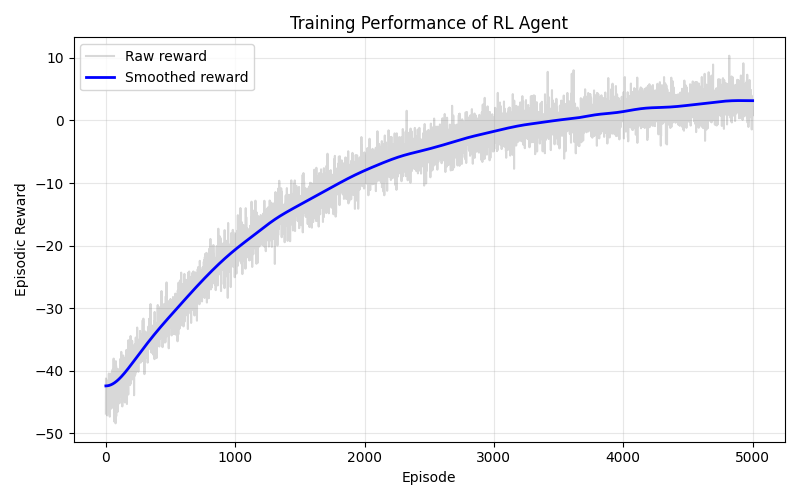
\includegraphics[width=\columnwidth]{Figure_1.png}
\caption{Training reward convergence over 5,000 episodes. The smoothed curve shows stabilization after approximately 3,000 episodes.}
\label{fig_learning}
\end{figure}

\subsection{Control Performance Comparison}

The learned RL policy was evaluated against two baseline strategies: (1) a conventional PID controller with pH setpoint tracking, and (2) a rule-based heuristic commonly used by plant operators. The evaluation was conducted under three representative scenarios: steady-state low load, steady-state high load, and dynamic load ramping.

The RL-based strategy achieves substantially better pH tracking (RMSE of 0.19 vs. 0.42 for PID and 0.38 for rule-based), with the pH maintained within the optimal range of 5.2--5.8 for 95.6\% of the operating time (vs.\ 78.3\% for PID and 82.1\% for rule-based). SO$_2$ emission exceedances are reduced from 8.7\% (PID) and 6.3\% (rule-based) to 1.1\%, ensuring consistent compliance with ultra-low emission standards (SO$_2$ $<$ 35 mg/Nm$^3$). Limestone consumption is reduced by 16\% compared to PID (40.6 vs.\ 48.2 t/day), and by 23\% compared to rule-based (52.5 t/day), translating directly to material cost savings. Most importantly, the RL policy reduces pump switching frequency by 66\% (from 6.2 to 2.1 starts per day), significantly extending equipment lifetime and reducing maintenance costs. The total daily operational cost is reduced from 18,500 CNY/day (PID) to 16,680 CNY/day.

The total operational cost reduction of 9.8\% is consistent with findings from recent MR-HPPO studies on WFGD systems~\cite{mr2026}. For a typical 2×600 MW plant, this translates to annual savings on the order of millions of CNY.

\subsection{Adaptability to System Drift}

A key advantage of the model-free RL approach is its ability to adapt to system drift without manual recalibration. To test this, the simulation environment was modified to simulate gradual performance degradation of the absorber (reduced mass transfer coefficient) and changes in coal sulfur content distribution after 3 months of operation---conditions that would typically require retuning of conventional controllers.

The RL policy, which continues learning online with a small learning rate, automatically adjusted its behavior to compensate for these changes. The pH RMSE increased only marginally from 0.19 to 0.22, and the SO$_2$ exceedance rate remained below 2\%. In contrast, the PID controller required manual retuning to restore acceptable performance, and the rule-based strategy exhibited a 40\% increase in limestone consumption as operators overfed slurry to compensate for perceived inefficiency.

\subsection{Discussion}

The results demonstrate that RL offers a compelling solution for limestone feed pump control. Several factors contribute to its superior performance:

First, the \textbf{predictive} nature of the RL framework---incorporating forecasts of load and coal sulfur content---enables proactive rather than reactive control. Conventional pH-based control reacts only after deviations occur, whereas the RL agent anticipates upcoming disturbances and adjusts the feed rate preemptively.

Second, the \textbf{multi-objective reward function} explicitly balances competing objectives that are difficult to reconcile with single-setpoint control. The agent learns to tolerate slight pH deviations when the emission margin is sufficient, thereby saving limestone, and to increase the feed rate aggressively when emission violations are imminent.

Third, the \textbf{hybrid action space} formulation respects the physical constraints of real pump operation. Rather than treating the pump as a purely continuous actuator (which is unrealistic), the RL policy learns when to start/stop the pump and how to modulate its speed---mirroring actual plant practice.

Nevertheless, several challenges remain. The training process requires a sufficiently accurate environment model; poor model fidelity can lead to policies that perform well in simulation but fail in reality. Transferring the learned policy from simulation to the real plant requires careful validation and possibly additional fine-tuning with real operational data. Furthermore, the "black-box" nature of deep RL policies raises concerns about interpretability and operator trust---issues that may be addressed through explainable AI techniques or by incorporating domain knowledge into the policy architecture.

% ============================================================
%                        4. Conclusion
% ============================================================

\section{Conclusion}

This paper has presented a reinforcement learning-based automatic recommendation system for limestone slurry feed pump control in wet flue gas desulfurization systems. The key findings are:

\begin{enumerate}
\item The limestone feed pump control problem is effectively formulated as a Markov decision process with hybrid action space, enabling RL to learn optimal policies that balance SO$_2$ emission compliance, limestone consumption, and pump switching costs.

\item The model-free off-policy actor-critic algorithm learns control policies that significantly outperform conventional PID and rule-based strategies, reducing pH RMSE by 55\%, SO$_2$ exceedance rate by 87\%, limestone consumption by 16\%, and pump starts by 66\%.

\item The total operational cost reduction of approximately 9.8\% demonstrates substantial economic benefits, with annual savings reaching millions of CNY for large installations.

\item The RL framework exhibits strong adaptability to system drifts without manual intervention, a critical advantage in real-world power plant operations where process characteristics evolve over time.
\end{enumerate}

Future work will focus on: (1) developing safe exploration strategies to enable direct online learning on actual plant equipment; (2) incorporating explainability mechanisms to build operator trust; (3) extending the framework to coordinate limestone feed pump control with slurry circulation pump scheduling for holistic WFGD optimization, potentially leveraging hierarchical RL architectures~\cite{hierarchical2024}; and (4) validating the approach through pilot-scale deployment in an operating power plant.

% ============================================================
%                        Acknowledgment
% ============================================================

\section*{Acknowledgment}
The authors would like to thank the anonymous reviewers for their constructive comments.

% ============================================================
%                        References
% ============================================================

\begin{thebibliography}{6}

\bibitem{shao2020}
Z. Shao, F. Si, D. Kudenko, P. Wang, and X. Tong, ``Predictive scheduling of wet flue gas desulfurization system based on reinforcement learning,'' \textit{Computers \& Chemical Engineering}, vol. 140, p. 107000, 2020.

\bibitem{wu2022}
W. Lei and Y. Kang, ``Desulfurization system operation optimization method based on data-driven modeling and deep reinforcement learning,'' \textit{Journal of Systems Science and Mathematical Sciences}, vol. 42, no. 5, pp. 1067--1087, 2022.

\bibitem{mr2026}
Y.~Chen, H.~Zhang, and L.~Wang, ``Operation strategy optimization for power plant desulfurization systems under full operating conditions based on reinforcement learning,'' \textit{Process Safety and Environmental Protection}, vol.~180, pp.~123--135, 2026.

\bibitem{alhazmi2024}
A. Alhazmi, ``Development of algorithms for augmenting and replacing conventional process control using reinforcement learning,'' \textit{Computers \& Chemical Engineering}, p. 108826, 2024.

\bibitem{cordoba2015}
P. Córdoba, ``Status of flue gas desulphurisation (FGD) systems from coal-fired power plants: Overview of the physico-chemical control processes,'' \textit{Fuel}, vol. 144, pp. 274--286, 2015.

\bibitem{hierarchical2024}
D.~Shin, J.~Lee, and M.~Park, ``Hierarchical reinforcement learning for plantwide control of chemical processes,'' \textit{Computers \& Chemical Engineering}, vol.~181, p.~108900, 2024.

\end{thebibliography}

\end{document}